\documentclass[12pt, a4paper]{article}

% --- Pakiety ---
\usepackage[utf8]{inputenc}
\usepackage[T1]{fontenc}
\usepackage[polish]{babel}
\usepackage{geometry}
\usepackage{amsmath}
\usepackage{amssymb}
\usepackage{graphicx}
\usepackage{booktabs}
\usepackage{siunitx}
\usepackage{caption}
\usepackage{subcaption}
\usepackage{float}
\usepackage{hyperref}
\usepackage{xcolor}
\usepackage{array}
\usepackage{multirow}
\usepackage{fancyhdr}

% --- Kropka ---
\captionsetup{labelsep=period}

% --- Marginesy ---
\geometry{
    top=2.5cm,
    bottom=2.5cm,
    left=2.5cm,
    right=2.5cm
}

% --- Stopka ---
\pagestyle{fancy}
\fancyhf{}
\renewcommand{\headrulewidth}{0pt}
\renewcommand{\footrulewidth}{0.4pt}
\fancyfoot[R]{
\includegraphics[height=0.8cm]{lumon.pdf}}

% --- Konfiguracja siunitx ---
\sisetup{
    output-decimal-marker = {,},
    separate-uncertainty = true
}

% --- Dane raportu ---
\newcommand{\tytul}{Badanie ruchu obrotowego bryły sztywnej}
\newcommand{\codeword}{Todos~Santos}
\newcommand{\nrCwiczenia}{M7}
\newcommand{\autor}{Karol Peszek}
\newcommand{\nrGrupy}{B1}
\newcommand{\dataWykonania}{1 kwietnia 2026}

% --- Tytuł dokumentu ---
\title{
    \large I Pracownia Fizyczna \\[0.5em]
    \textbf{Ćwiczenie \nrCwiczenia} \\[0.3em]
    \LARGE \tytul\space''\codeword''
}
\author{
    \autor\\
     Grupa \nrGrupy}
\date{
    Data wykonania pomiarów: \dataWykonania\\
}

% =============================================
\begin{document}
% =============================================

\maketitle
\thispagestyle{empty}
\newpage

% -------------------------------------------
\section{Cel ćwiczenia}
% -------------------------------------------
W niniejszej pracy zbadano ruch obrotowy bryły sztywnej na przykładzie wahadła Oberbecka napędzanego układem ciężarków zawieszonych na nici nawiniętej na oś wahadła. Przeprowadzono trzy serie pomiarowe, w których systematycznie zmieniano odległość bramek fotoelektrycznych, odległość ciężarków walcowych od osi obrotu oraz masę ciężarków napędowych, rejestrując każdorazowo czas przelotu między bramkami. Na podstawie ważonej regresji liniowej wyznaczono moment bezwładności wahadła nieobciążonego $J_X$ z trzech niezależnych eksperymentów i porównano uzyskane wartości. Wyniki potwierdzają liniowość przewidzianych przez teorię zależności oraz pozostają ze sobą w zgodności w granicach wyznaczonych niepewności pomiarowych.

% -------------------------------------------
\section{Wstęp teoretyczny}
% -------------------------------------------

\subsection{Bryła sztywna}
Bryła sztywna to wyidealizowany model fizyczny zakładający ciało składające się z infinitezymalnie małych elementów, które są ze sobą połączone w taki sposób, że odległości między nimi pozostają stałe podczas ruchu. Oznacza to, że bryła sztywna nie ulega odkształceniom ani rozciąganiu pod wpływem sił działających na nią.

\subsection{Środek masy i moment bezwładności}
Środek masy bryły sztywnej to punkt, w którym można wyobrazić sobie skoncentrowaną całą masę ciała. Formalnie środek masy jest punktem w trójwymiarowej przestrzeni opisanym przez wektor \(\vec{R}\), który jest średnią ważoną położenia wszystkich elementów masy ciała:
\begin{equation}
    \vec{R} = \frac{1}{M} \sum_{i} m_i \vec{r}_i
\end{equation}
gdzie \(M\) to całkowita masa bryły, \(m_i\) to masa i-tego elementu, a \(\vec{r}_i\) to jego położenie.
W przypadku ciągłym sumę należy zastąpić całką:
\begin{equation}
    \vec{R} = \frac{1}{M} \int \vec{r} \, dm
\end{equation}

Moment bezwładności jest skalarną wielkością mówiącą jaki moment siły należby przyłożyć do ciała aby uzyskać określone przyspieszenie kątowe. Dla bryły sztywnej moment bezwładności \(I\) względem osi obrotu jest definiowany jako:
\begin{equation}
    I = \sum_{i} m_i r_i^2
\end{equation}
gdzie \(r_i\) to odległość i-tego elementu masy od osi obrotu. W przypadku ciągłym, moment bezwładności można wyrazić jako całkę:
\begin{equation}
    I = \int r^2 \, dm
\end{equation} 

\subsection{Dynamika ruchu obrotowego}

Jeżeli wypadkowy moment siły działający na bryłę sztywną wynosi zero, to bryła pozostaje w spoczynku lub obraca się ruchem jednostajnym (ze stałą prędkością kątową). Pod działaniem momentu siły $\vec{N}$ bryła sztywna może wykonywać ruch obrotowy. Do opisu ruchu obrotowego używa się kąta $\vec{\phi}$ o jaki obraca się bryła, prędkości kątowej $\vec{\omega} = d\vec{\phi}/dt$, przyspieszenia kątowego $\vec{\varepsilon} = d^2\vec{\phi}/dt^2$ oraz momentu pędu $\vec{L}$. Równanie opisujące ruch obrotowy wokół osi $O$ bryły sztywnej o momencie bezwładności $J_{(O)}$ ma postać:
\begin{equation}
    \vec{N} = J_{(O)} \frac{d^2\vec{\phi}}{dt^2},
    \label{eq:rotational_motion}
\end{equation}
lub, zapisane przy użyciu momentu pędu:
\begin{equation}
    \vec{N} = \frac{d\vec{L}}{dt}.
\end{equation}
Najprostszym przykładem ruchu obrotowego jest obrót bryły sztywnej dookoła ustalonej osi. Wtedy wektory momentu siły $\vec{N}$, prędkości kątowej $\vec{\omega}$ oraz momentu pędu $\vec{L} = J_{(O)}\vec{\omega}$ są do siebie równoległe i powiązane poprzez równanie ruchu:
\begin{equation}
    \vec{N} = \frac{d\vec{L}}{dt} = J_{(O)} \frac{d\vec{\omega}}{dt}.
\end{equation}
W ogólnym przypadku wektor momentu pędu bryły sztywnej nie jest równoległy do wektora prędkości kątowej. Wtedy wielkości te powiązane są ze sobą przez:
\begin{equation}
    \vec{L} = \hat{J}\vec{\omega},
\end{equation}
gdzie tensor bezwładności $\hat{J}$ jest tensorem symetrycznym drugiego rzędu. Tensor bezwładności można zawsze zdiagonalizować poprzez obrót układu współrzędnych --- osie tego nowego układu współrzędnych nazywane są \textit{głównymi osiami bezwładności}.

\subsection{Twierdzenie Steinera}
Moment bezwładności względem osi przechodzącej przez środek masy oblicza się z definicji. Dla określenia momentu bezwładności względem innej osi korzysta się z \textit{twierdzenia o osiach równoległych} (twierdzenie Steinera).

Oznaczmy przez $J_{CM}$ moment bezwładności bryły względem osi $O_{CM}$ przechodzącej przez środek masy. Moment bezwładności $J_{(O)}$ względem osi $O$ równoległej do $O_{CM}$ wyraża się wzorem:
\begin{equation}
    J_{(O)} = J_{CM} + Md^2,
    \label{eq:steiner}
\end{equation}
gdzie $d$ to wzajemna odległość osi $O$ i $O_{CM}$, a $M$ to masa bryły.

Dla jednorodnego walca o masie $M$, promieniu $R$ i wysokości $H$ środek masy leży na osi symetrii obrotowej, w połowie wysokości. Moment bezwładności względem osi pokrywającej się z osią symetrii wynosi $J_{CM} = \frac{1}{2}MR^2$, natomiast względem osi do niej prostopadłej przechodzącej przez środek masy:
\begin{equation}
    J_{CM} = M\!\left(\frac{1}{4}R^2 + \frac{1}{12}H^2\right).
    \label{eq:cylinder_perp}
\end{equation}

\subsection{Wahadło Oberbecka}

Wahadło Oberbecka jest bryłą sztywną obracającą się wokół poziomej osi, składającą się z prostopadłych do siebie par ramion. Do ramion można przyczepić ciężarki w kształcie walca (masa $M_W$, promień $R_W$, wysokość $H_W$).
Walec umieszczony jest w odległości $d_W$ od osi obrotu wahadła Oberbecka. Korzystając z twierdzenia Steinera (wzór~\ref{eq:steiner}), obliczamy moment bezwładności walca względem tej osi:
\begin{equation}
    J_W = J_{W,CM} + M_W d_W^2.
\end{equation}

Moment bezwładności nieobciążonego wahadła wynosi $J_X$. Przy obciążeniu dwoma identycznymi ciężarkami umieszczonymi symetrycznie w odległości $d_W$ od osi, całkowity moment bezwładności układu wynosi $J = J_X + 2J_W$.

Na osi wahadła o promieniu $r$ nawinięta jest nić, która przechodzi przez bloczek i zakończona jest szalką z ciężarkami o masie $m$. Równanie ruchu postępowego ciężarka zawieszonego na nici ma postać:
\begin{equation}
    mg - F_N = m\frac{d^2x}{dt^2},
    \label{eq:translational}
\end{equation}
gdzie $F_N$ to siła naciągu nici, a $x$ to droga przebyta przez ciężarek. Na wahadło działa moment siły $N = F_N r$, więc równanie ruchu obrotowego wahadła ma postać:
\begin{equation}
    \left(J_X + 2J_W\right)\frac{d^2\phi}{dt^2} = F_N r.
    \label{eq:rotational_pendulum}
\end{equation}
Zmienne $x$ i $\phi$ są ze sobą związane zależnością $x = r\phi$, skąd $d^2x/dt^2 = r\,d^2\phi/dt^2$. Korzystając z równań (\ref{eq:translational}) i (\ref{eq:rotational_pendulum}), obliczamy przyspieszenie układu:
\begin{equation}
    a = \frac{d^2x}{dt^2} = \frac{mgr^2}{J_X + 2J_W + mr^2}.
    \label{eq:acceleration}
\end{equation}
Dla ruchu jednostajnie przyspieszonego ciężarka startującego ze spoczynku droga wynosi $x(t) = at^2/2$, co pozwala na weryfikację praw ruchu obrotowego poprzez pomiary czasu przelotu~\cite{skrypt}.

% -------------------------------------------
\section{Opis układu pomiarowego}
% -------------------------------------------

\subsection{Wahadło Oberbecka}
Używane w pomiarach wahadło Oberbecka (Rysunek~\ref{fig:oberbeck}.) jest obracającym się wokół poziomej osi układem dwóch par ramion. Do ramion można przyczepić ciężarki walcowe ($M_W$, $R_W$, $H_W$) umieszczane symetrycznie po obu stronach osi obrotu w odległości $d_W$. Na osi wahadła o promieniu $r$ nawinięta jest nić, która przechodzi przez bloczek i zakończona jest szalką z ciężarkami o masie $m$. Do pomiaru czasu przelotu szalki między ustalonymi punktami używane są bramki elektroniczne (fotokomórki).

\begin{figure}[H]
    \centering
    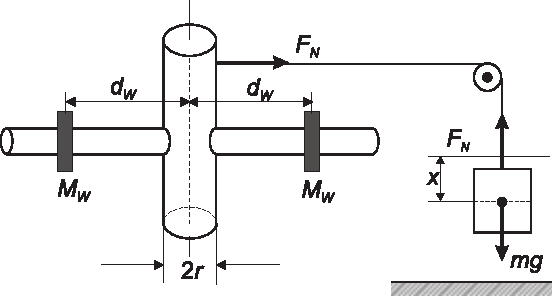
\includegraphics[width=0.82\textwidth]{oberbeck_pendulum.pdf}
    \caption{Schemat układu doświadczalnego z wahadłem Oberbecka. $M_W$ --- masy ciężarków walcowych, $d_W$ --- odległość ciężarków od osi obrotu, $2r$ --- średnica osi nawijania nici, $F_N$ --- siła naciągu nici, $x$ --- droga ciężarka, $mg$ --- siła ciężkości. Źródło:~\cite{skrypt}.}\label{fig:oberbeck}
\end{figure}


\begin{figure}[H]
    \centering
    
\includegraphics[width=0.82\textwidth]{schema.jpg}
    \caption{Zdjęcie układu doświadczalnego z wahadłem Oberbecka.}\label{fig:oberbeck_photo}
\end{figure}

\subsection{Dostępne przyrządy}
Do dyspozycji były następujące przyrządy pomiarowe: wahadło Oberbecka z~możliwością montażu ciężarków walcowych, zestaw obciążników walcowych o~różnych masach, promieniach i~wysokościach, ciężarki do zawieszenia na nitce, fotokomórki do pomiaru czasu przelotu ciężarków, linijka do pomiaru wymiarów ciężarków i~odległości z~dokładnością \qty{1}{\mm}, waga elektryczna AXIS B2 o~zakresie pomiarowym do \qty{2000}{\gram} i~dokładności \qty{0.1}{\gram}, taśma miernicza do pomiaru odległości między fotokomórkami o~dokładności \qty{1}{\mm} oraz suwmiarka do pomiaru wymiarów ciężarków walcowych i~ich odległości od osi obrotu o~dokładności \qty{0.1}{\mm}.
% -------------------------------------------
\section{Procedura pomiarowa}
% -------------------------------------------

We wszystkich trzech seriach eksperymentalnych zastosowano jednolitą procedurę pomiarową, różniącą się jedynie parametrem zmienianym między seriami. W każdym przypadku fotokomórki ustawiano w zadanej odległości od siebie, po czym na szalce zawieszano ciężarki o odpowiednio dobranej masie $m$. Przed każdym pomiarem obracano wahadło powoli w kierunku nawijania nitki, tak aby ciężarek znalazł się ponad górną fotokomórką i ją aktywował, co służyło jako punkt zerowania układu mierzącego czas. Następnie cofano ciężarek do pozycji startowej, zerowano fotokomórkę i zwalniano wahadło, rejestrując czas swobodnego spadku ciężarków między fotokomórkami. Czynność tę powtarzano 10-krotnie w obrębie każdej serii, a do dalszych obliczeń wykorzystano średni czas przelotu. Różnica między poszczególnymi seriami polegała wyłącznie na tym, który parametr był zmieniany: w pierwszej serii zmieniano odległość fotokomórek przy braku ciężarków walcowych na ramionach, w drugiej serii zmieniano odległość ciężarków walcowych od osi obrotu przy stałej odległości fotokomórek, natomiast w trzeciej serii zmieniano masę ciężarków zawieszonych na nitce przy stałej odległości fotokomórek i braku ciężarków walcowych. We wszystkich seriach parametry niezmieniane były utrzymywane na stałym poziomie przez cały czas trwania danej serii.


% -------------------------------------------
\section{Wyniki pomiarów}
% -------------------------------------------
Dla każdej z trzech zależności przeprowadzono 4 serie pomiarowe, każda po 10 pomiarów. Poniżej przedstawiono zebrane dane pomiarowe w formie tabelarycznej oraz graficznej.

\subsection{Zależność kwadratu czasu przelotu od odległości fotokomórek}

\begin{table}[H]
    \centering
    \caption{Średnie czasy przelotu $\langle t \rangle$ i odchylenia standardowe $\sigma(t)$ dla czterech odległości bramek $h$ (10 pomiarów każda seria).}\label{tab:t_vs_h}
    \begin{tabular}{S[table-format=2.0] S[table-format=1.4] S[table-format=1.4]}
        \toprule
        {$h$ (cm)} & {$\langle t \rangle$ (s)} & {$\sigma(t)$ (s)} \\
        \midrule
        20 & 3.8864 & 0.0556 \\
        30 & 4.9450 & 0.0646 \\
        40 & 5.8680 & 0.0251 \\
        50 & 6.5354 & 0.0789 \\
        \bottomrule
    \end{tabular}
\end{table}

\begin{figure}[H]
    \centering
    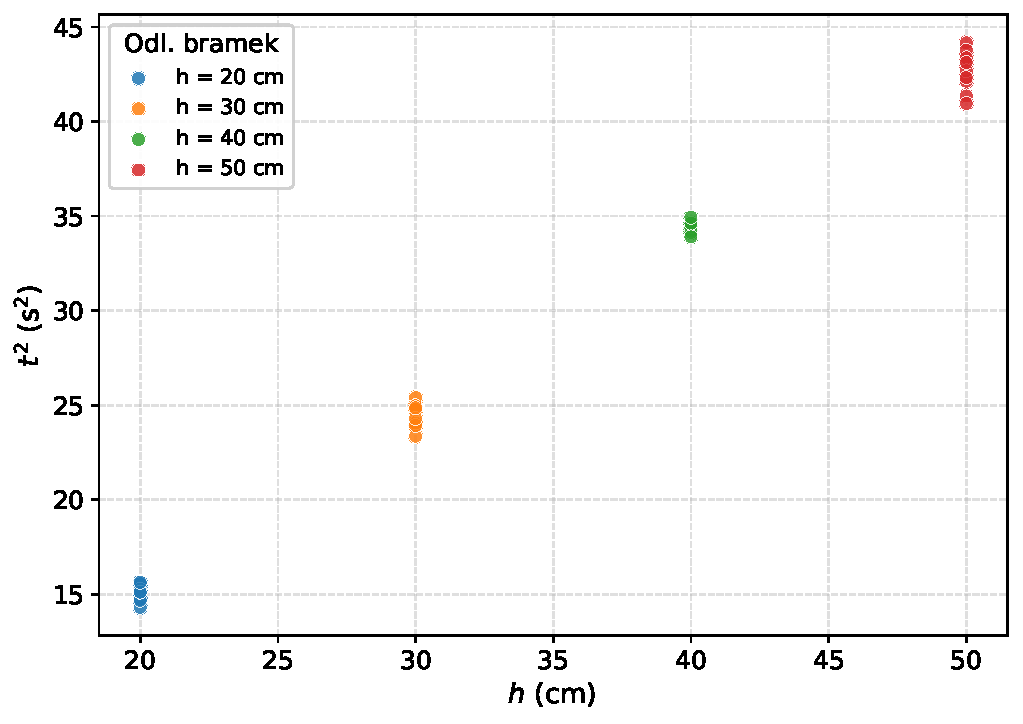
\includegraphics[width=0.82\textwidth]{wykres1_surowe_h.pdf}
    \caption{Pomiary $t^2$ w funkcji odległości bramek $h$ dla czterech serii pomiarowych.}\label{fig:surowe_h}
\end{figure}

\subsection{Zależność kwadratu czasu przelotu od kwadratu odległości ciężarków od osi obrotu}

\begin{table}[H]
    \centering
    \caption{Średnie czasy przelotu $\langle t \rangle$ i odchylenia standardowe $\sigma(t)$ dla czterech odległości ciężarków walcowych $r_W$ od osi obrotu (10 pomiarów każda seria). Wielkość $d_t$ to odległość między zewnętrznymi krawędziami obu walców zamontowanych symetrycznie po obu stronach osi, mierzona suwmiarką. Z symetrii układu odległość od osi do zewnętrznej krawędzi jednego walca wynosi $d_t/2$, a odległość od osi do środka masy walca (odległość wzdłuż ramienia wynosi $H_W/2$) wynosi $r_W = d_t/2 - H_W/2 = (d_t - H_W)/2$, gdzie $H_W = \qty{10.0}{mm}$.}\label{tab:t_vs_rw}
    \begin{tabular}{S[table-format=3.2] S[table-format=1.4] S[table-format=1.4]}
        \toprule
        {$r_W$ (mm)} & {$\langle t \rangle$ (s)} & {$\sigma(t)$ (s)} \\
        \midrule
        44.95 & 3.7135 & 0.0580 \\
        84.25 & 4.1591 & 0.0737 \\
        124.30 & 4.7851 & 0.0752 \\
        164.50 & 5.5523 & 0.1024 \\
        \bottomrule
    \end{tabular}
\end{table}

\begin{figure}[H]
    \centering
    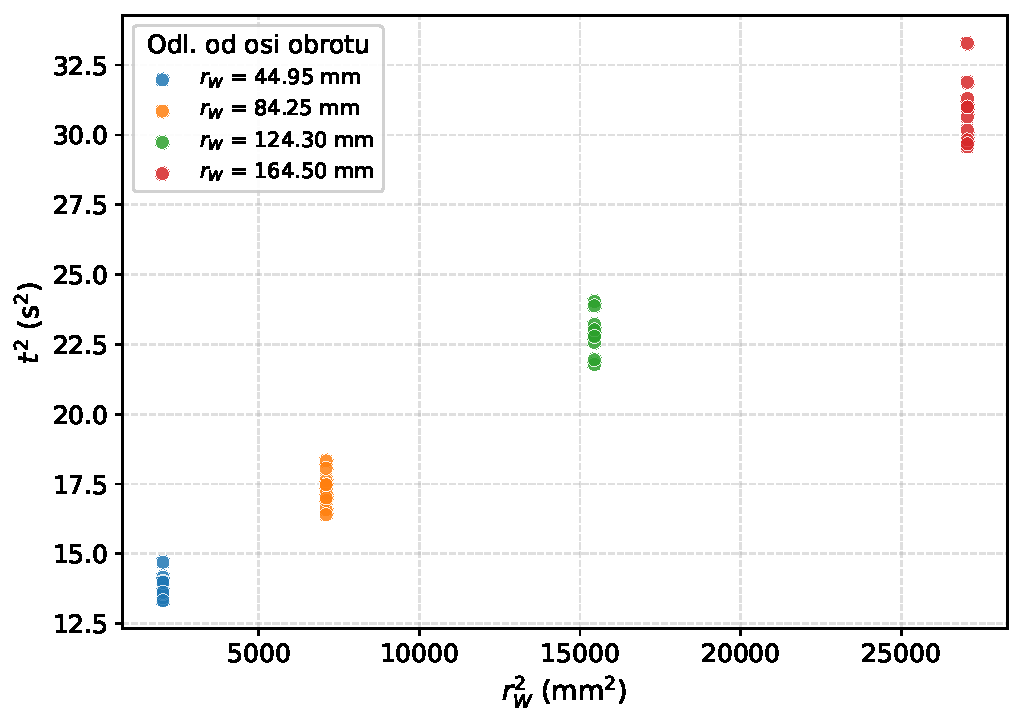
\includegraphics[width=0.82\textwidth]{wykres2_surowe_dw2.pdf}
    \caption{Pomiary $t^2$ w funkcji $r_W^2$ dla czterech odległości ciężarków walcowych od osi obrotu.}\label{fig:surowe_dw2}
\end{figure}

\subsection{Zależność kwadratu czasu przelotu od odwrotności masy ciężarków na nitce}

\begin{table}[H]
    \centering
    \caption{Średnie czasy przelotu $\langle t \rangle$ i odchylenia standardowe $\sigma(t)$ dla czterech mas ciężarków zawieszonych na nitce (10 pomiarów każda seria).}\label{tab:t_vs_m}
    \begin{tabular}{S[table-format=3.1] S[table-format=1.4] S[table-format=1.4]}
        \toprule
        {$m$ (g)} & {$\langle t \rangle$ (s)} & {$\sigma(t)$ (s)} \\
        \midrule
        99.8  & 4.9450 & 0.0646 \\
        119.7 & 4.5336 & 0.0711 \\
        139.6 & 4.1999 & 0.0799 \\
        159.6 & 3.9202 & 0.0594 \\
        \bottomrule
    \end{tabular}
\end{table}

\begin{figure}[H]
    \centering
    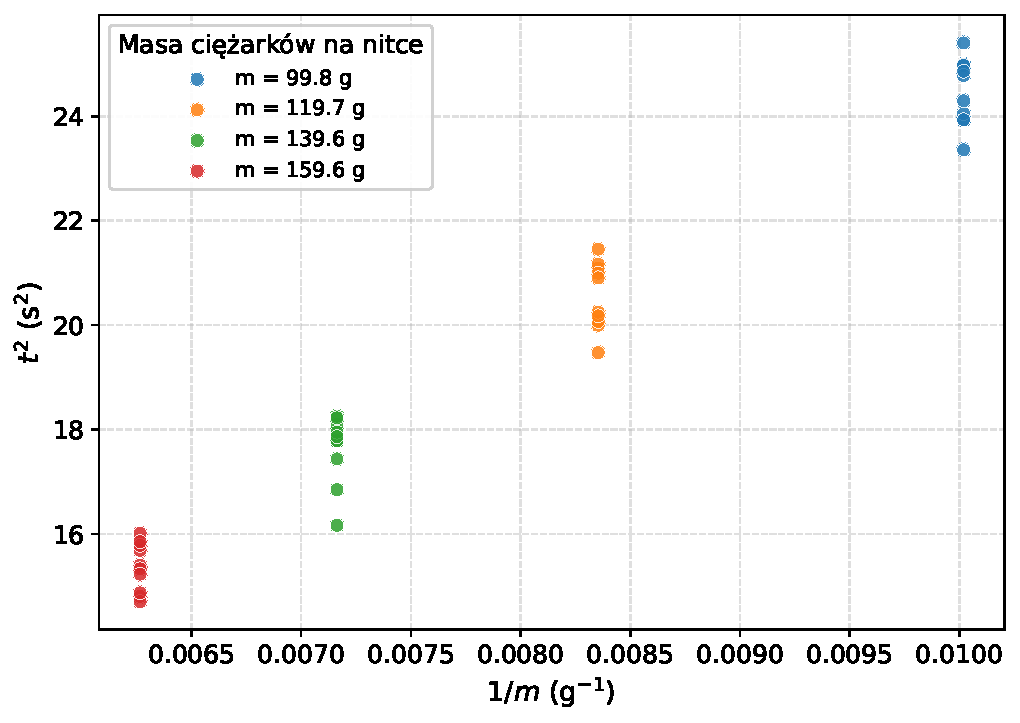
\includegraphics[width=0.82\textwidth]{wykres3_surowe_m.pdf}
    \caption{Pomiary $t^2$ w funkcji $1/m$ dla czterech mas ciężarków zawieszonych na nitce.}\label{fig:surowe_m}
\end{figure}


% -------------------------------------------
\section{Rachunek niepewności}
% -------------------------------------------

\subsection{Niepewności pomiarów bezpośrednich}

Niepewności przyrządów pomiarowych przyjęto jako:
\begin{itemize}
    \item waga: $u(m) = \qty{0.1}{\g}$,
    \item suwmiarka: $u(d) = \qty{0.1}{\mm}$,
    \item taśma miernicza: $u(h) = \qty{1}{\mm}$.
\end{itemize}
Niepewność promienia szpuli $u(r)$ wyznaczono z prawa propagacji dla $r = D_s/2$:
$u(r) = u(D_s)/2$.

\subsection{Niepewności współczynników regresji}

We wszystkich trzech eksperymentach użyto ważonej regresji liniowej z wagami $w_i = 1/\sigma_i^2$, gdzie $\sigma_i$ jest odchyleniem standardowym $t^2$ w $i$-tej serii (10 powtórzeń). Macierz kowariancji współczynników wyznaczono analitycznie jako ${(A^{T}WA)}^{-1}$, co daje niepewności:
\[
    u(a) = \sqrt{{[{({A^T}WA)}^{-1}]}_{11}}, \qquad u(b) = \sqrt{{[{({A^T}WA)}^{-1}]}_{22}}.
\]
Niepewność prostej regresji w punkcie $x$ wyznaczono z prawa propagacji:
\[
    u(y_{\text{fit}}(x)) = \sqrt{u^2(a)\,x^2 + u^2(b)}.
\]

\subsection{Niepewności momentu bezwładności}

Niepewności $J_X$ wyznaczono metodą propagacji niepewności.

\paragraph{Eksperyment 1.} Ze wzoru $J_X = \tfrac{1}{2}A_1 m_1 g r^2 - m_1 r^2$:
\[
    u(J_X) = \sqrt{
        {\left(\frac{m_1 g r^2}{2}\right)}^2 u^2(A_1)
        + {\left(m_1 r\!\left(A_1 g - 2\right)\right)}^2 u^2(r)
        + {\left(r^2\!\left(\frac{A_1 g}{2} - 1\right)\right)}^2 u^2(m_1)
    }.
\]

\paragraph{Eksperyment 2.} Ze wzoru $J_X = B_2 m_2 g r^2/(2h_2) - J_{W,0} - m_2 r^2$, gdzie $J_{W,0} = M_W(R_W^2/4 + H_W^2/12)$:
\begin{align*}
    u^2(J_X) =
        &{\left(\frac{m_2 g r^2}{2h_2}\right)}^2\!u^2(B_2)
        +{\left(\frac{B_2 m_2 g r^2}{2h_2^2}\right)}^2\!u^2(h_2) \\
        &+{\left(\frac{B_2 m_2 g r}{h_2}\right)}^2\!u^2(r)
        +{\left(\frac{B_2 g r^2}{2h_2}\right)}^2\!u^2(m_2) \\
        &+{\left(\frac{R_W^2}{4} + \frac{H_W^2}{12}\right)}^2\!u^2(M_W)
        +{\left(\frac{M_W R_W}{2}\right)}^2\!u^2(R_W)
        +{\left(\frac{M_W H_W}{6}\right)}^2\!u^2(H_W).
\end{align*}

\paragraph{Eksperyment 3.} Ze wzoru $J_X = A_3 g r^2 / (2h_3)$:
\[
    u(J_X) = \sqrt{
        {\left(\frac{g r^2}{2h_3}\right)}^2 u^2(A_3)
        + {\left(\frac{A_3 g r}{h_3}\right)}^2 u^2(r)
        + {\left(\frac{A_3 g r^2}{2h_3^2}\right)}^2 u^2(h_3)
    }.
\]

\subsection{Źródła błędów systematycznych}

Przyjęty model zakłada ruch bez oporów i pewne idealizacje, które w rzeczywistości nie są spełnione. Poniżej omówiono główne źródła błędów systematycznych.

\begin{description}
    \item[Opór powietrza.] Siła oporu aerodynamicznego spowalnia zarówno spadające ciężarki, jak i obracające się ramiona wahadła, zmniejszając efektywne przyspieszenie układu. Powoduje to systematyczne zawyżenie mierzonych czasów przelotu.

    \item[Tarcie w łożyskach wahadła.] Tarcie w osi obrotu wahadła działa jak dodatkowy moment hamujący, nieuwzględniony w modelu. Analogicznie jak opór powietrza, wydłuża czasy przelotu i prowadzi do zawyżenia wyznaczonego $J_X$.

    \item[Kołysanie wahadła na stojaku.] Jeśli stojak nie jest dostatecznie sztywny lub wahadło nie jest wyważone, ramiona mogą się kołysać w płaszczyźnie poprzecznej do osi obrotu. Taki ruch odbiera energię układowi, zaburza mierzone czasy i zwiększa ich rozrzut między powtórzeniami.

    \item[Rozciąganie się nitki.] Przy obciążeniu nitka wydłuża się sprężyście, zmniejszając efektywny promień nawijania $r$ w stosunku do wartości zmierzonej suwmiarką na nieobciążonej osi. Zaniżenie $r$ prowadzi do błędu systematycznego w wyznaczanym momencie bezwładności.

    \item[Tarcie nitki i moment bezwładności bloczka.] Model zakłada, że bloczek zmienia jedynie kierunek nici i nie pochłania energii. W rzeczywistości tarcie nitki o rowek bloczka oraz moment bezwładności samego bloczka zmniejszają przyspieszenie układu. Skutek jest analogiczny do tarcia w osi wahadła.

    \item[Wahania nitki z ciężarkami.] Jeśli ciężarki nie są puszczane pionowo, nić z szalką może się wahać jak wahadło. Zaburza to ruch postępowy ciężarków i powoduje niepowtarzalność warunków startowych między kolejnymi pomiarami, zwiększając odchylenie standardowe w obrębie serii.

    \item[Niezerowa prędkość startowa ciężarka.] Model zakłada start ze spoczynku ($v_0 = 0$). Jeśli ciężarek jest zwalniany z niezerową prędkością lub jeśli fotokomórka nie jest aktywowana dokładnie w momencie zatrzymania (wyzerowania), do pomiaru wchodzi dodatkowy składnik kinematyczny. Systematyczne zawyżenie lub zaniżenie $t$ przekłada się bezpośrednio na błąd $t^2$.
\end{description}

% -------------------------------------------
\section{Opracowanie wyników}
% -------------------------------------------
We wszystkich przypadkach wyznaczono średnie i standardowe odchylenia $t^2$ dla każdej serii pomiarowej.
Następnie użyto modelu ważonej regresji liniowej (wagi $w_i = 1/\sigma_i^2$) do dopasowania współczynników w zależności liniowej $t^2 = a x + b$, gdzie $x$ to odpowiednio $h$, $r_W^2$ lub $1/m$.
\subsection{Zależność kwadratu czasu przelotu od odległości fotokomórek}

Bez ciężarków walcowych ($J_W = 0$) i przy stałej masie szalki $m_1$, podstawiając $x = h$ do wzoru~(\ref{eq:acceleration}) z warunkiem $t^2 = 2h/a$, otrzymujemy model liniowy:
\begin{equation}
    t^2 = A_1 \cdot h + B_1, \qquad A_1 = \frac{2(J_X + m_1 r^2)}{m_1 g r^2}.
    \label{eq:model1}
\end{equation}
Ważona regresja liniowa (wagi $w_i = 1/\sigma_i^2$, gdzie $\sigma_i$ to odchylenie standardowe $t^2$ w danej serii) dała wyniki przedstawione na rysunku~\ref{fig:reg_h}:
\begin{align*}
    A_1 &= \qty{95.6 \pm 2.4}{\s\squared\per\m}, \\
    B_1 &= \qty{-3.98 \pm 0.84}{\s\squared}, \\
    R^2 &= 0{,}9990.
\end{align*}
\begin{figure}[H]
    \centering
    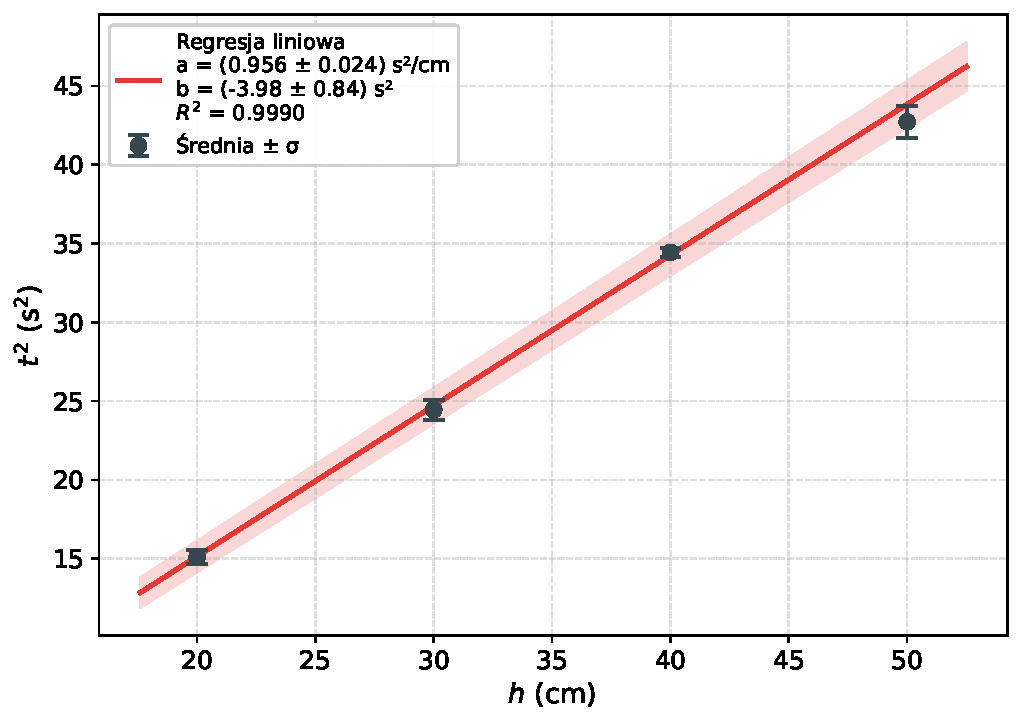
\includegraphics[width=0.82\textwidth]{wykres4_regresja_h.pdf}
    \caption{Regresja liniowa $t^2$ w funkcji odległości bramek $h$. Linia ciągła --- dopasowanie, zacieniony obszar --- niepewność prostej wynikająca z $u(A_1)$ i $u(B_1)$.}\label{fig:reg_h}
\end{figure}
Ze wzoru~(\ref{eq:model1}) wyznaczamy moment bezwładności wahadła:
\begin{equation}
    J_X = \frac{A_1 m_1 g r^2}{2} - m_1 r^2.
\end{equation}
Podstawiając wartości $m_1 = \qty{99.8 \pm 0.1}{\g}$, $g = \qty{9.81}{\m\per\s\squared}$, $r = \qty{10.05}{\mm}$:
\[
    \boxed{J_X = (4{,}72 \pm 0{,}13) \times 10^{-3}\ \si{\kg\m\squared}.}
\]

\subsection{Zależność kwadratu czasu przelotu od kwadratu odległości ciężarków od osi obrotu}

Wielkość $r_W$ oznacza odległość środka masy walca od osi obrotu. Zmierzono suwmiarką odległość $d_t$ między zewnętrznymi krawędziami obu walców (zamontowanych symetrycznie), skąd $r_W = d_t/2 - H_W/2 = (d_t - H_W)/2$.

Przy stałej odległości bramek $h_2 = \qty{30.0 \pm 0.1}{\cm}$ i stałej masie szalki $m_2$ moment bezwładności ciężarków $J_W = J_{W,0} + M_W r_W^2$ (twierdzenie Steinera, równanie~\ref{eq:steiner}), skąd model liniowy:
\begin{equation}
    t^2 = A_2 \cdot r_W^2 + B_2, \qquad
    A_2 = \frac{2h_2 M_W}{m_2 g r^2}, \quad
    B_2 = \frac{2h_2(J_X + J_{W,0} + m_2 r^2)}{m_2 g r^2}.
    \label{eq:model2}
\end{equation}
Przy zmierzonej odległości bramek $h_2$ moment bezwładności wyznaczamy bezpośrednio z wyrazu wolnego $B_2$:
\begin{equation}
    J_X = \frac{B_2\, m_2\, g\, r^2}{2h_2} - J_{W,0} - m_2 r^2.
\end{equation}
Ważona regresja liniowa dała wyniki przedstawione na rysunku~\ref{fig:reg_dw2}:
\begin{align*}
    A_2 &= \qty{680 \pm 42}{\s\squared\per\m\squared}, \\
    B_2 &= \qty{12.43 \pm 0.44}{\s\squared}, \\
    R^2 &= 1{,}0000.
\end{align*}
\begin{figure}[H]
    \centering
    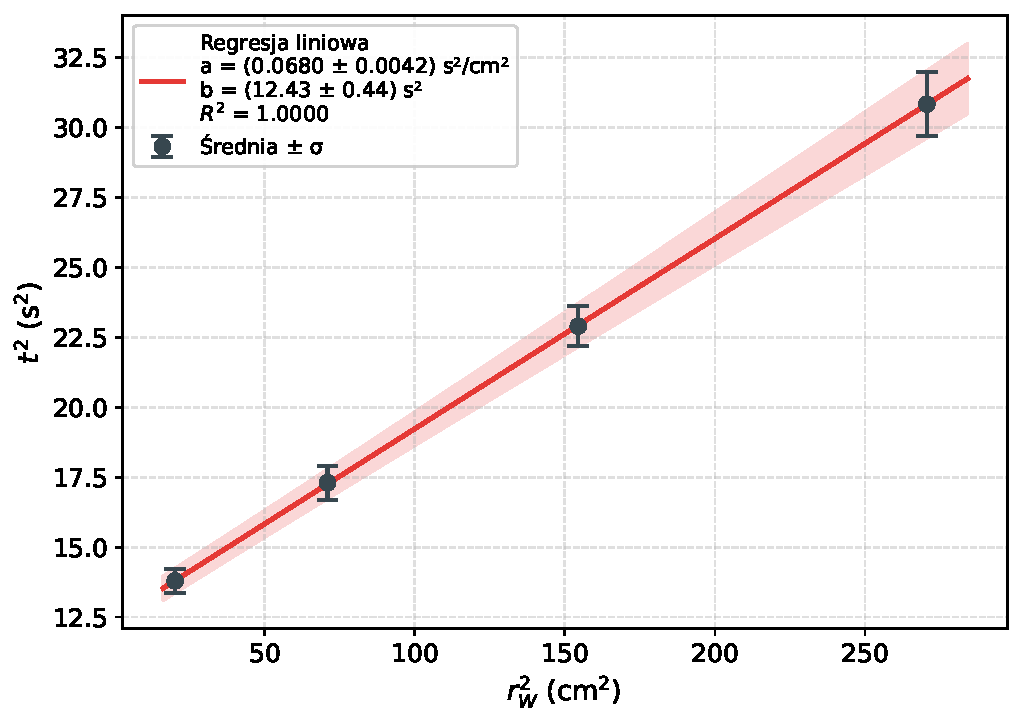
\includegraphics[width=0.82\textwidth]{wykres5_regresja_dw2.pdf}
    \caption{Regresja liniowa $t^2$ w funkcji $r_W^2$. Linia ciągła --- dopasowanie, zacieniony obszar --- niepewność prostej.}\label{fig:reg_dw2}
\end{figure}
Podstawiając zmierzone wartości:
\begin{itemize}
    \item masa szalki: $m_2 = \qty{199.4 \pm 0.1}{\g}$,
    \item łączna masa obu walców: $M_W = \qty{123.8 \pm 0.3}{\g}$,
    \item promień walca: $R_W = \qty{22.95 \pm 0.05}{\mm}$ (ze średnicy $d_W = \qty{45.9 \pm 0.1}{\mm}$),
    \item grubość walca: $H_W = \qty{10.0 \pm 0.1}{\mm}$,
    \item promień szpuli: $r = \qty{10.05 \pm 0.05}{\mm}$,
\end{itemize}
moment własny układu dwóch walców wynosi $J_{W,0} = M_W(R_W^2/4 + H_W^2/12) = \qty{0.0173e-3}{\kg\m\squared}$. Stąd:
\[
    \boxed{J_X = (4{,}06 \pm 0{,}15) \times 10^{-3}\ \si{\kg\m\squared}.}
\]

\subsection{Zależność kwadratu czasu przelotu od odwrotności masy ciężarków zawieszonych na nitce}

Bez ciężarków walcowych ($J_W = 0$), przy stałej odległości bramek $h_3$, model liniowy ma postać:
\begin{equation}
    t^2 = A_3 \cdot \frac{1}{m} + B_3, \qquad
    A_3 = \frac{2h_3 J_X}{g r^2}, \quad
    B_3 = \frac{2h_3}{g}.
    \label{eq:model3}
\end{equation}
Moment bezwładności wynika bezpośrednio ze współczynnika kierunkowego:
\begin{equation}
    J_X = \frac{A_3 g r^2}{2 h_3}.
\end{equation}
Ważona regresja liniowa dała wyniki przedstawione na rysunku~\ref{fig:reg_m}:
\begin{align*}
    A_3 &= \qty{2.42 \pm 0.20}{\s\squared\kg}, \\
    B_3 &= \qty{0.2 \pm 1.6}{\s\squared}, \\
    R^2 &= 0{,}9997.
\end{align*}
\begin{figure}[H]
    \centering
    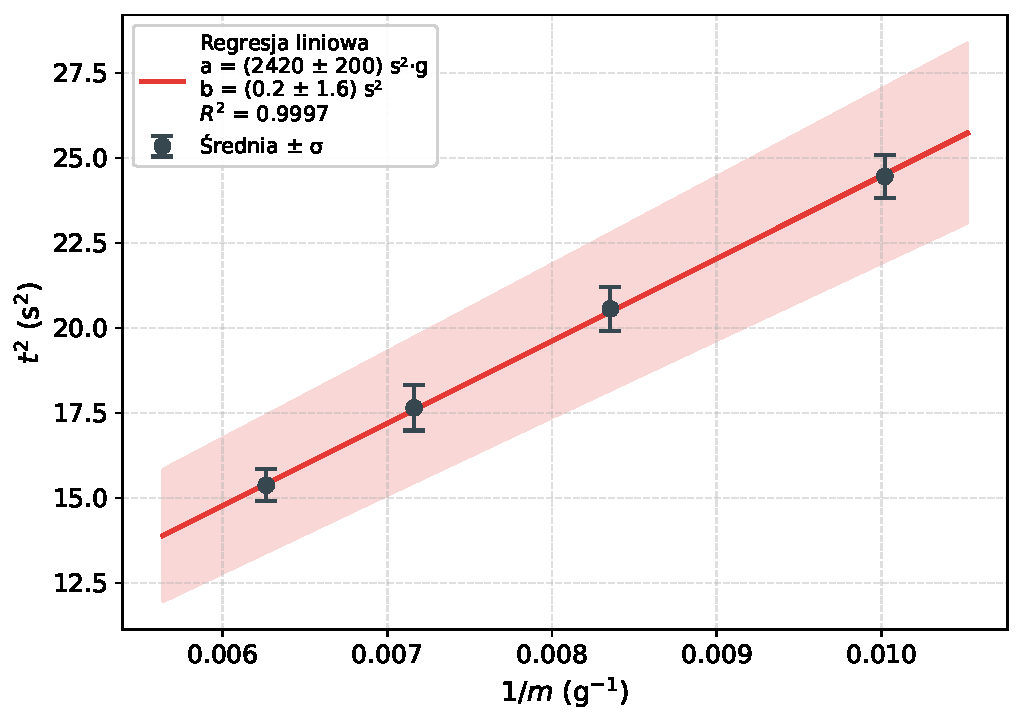
\includegraphics[width=0.82\textwidth]{wykres6_regresja_m.pdf}
    \caption{Regresja liniowa $t^2$ w funkcji $1/m$. Linia ciągła --- dopasowanie, zacieniony obszar --- niepewność prostej.}\label{fig:reg_m}
\end{figure}
Podstawiając $h_3 = \qty{30.0 \pm 0.1}{\cm}$:
\[
    \boxed{J_X = (4{,}00 \pm 0{,}34) \times 10^{-3}\ \si{\kg\m\squared}.}
\]

% -------------------------------------------
\section{Wnioski}
% -------------------------------------------

Zestawienie wyznaczonych wartości momentu bezwładności wahadła Oberbecka z trzech niezależnych eksperymentów:
\begin{table}[H]
    \centering
    \caption{Zestawienie wyników $J_X$ z trzech eksperymentów.}\label{tab:jx}
    \begin{tabular}{l S[table-format=1.2] @{${}\pm{}$} S[table-format=1.2] l}
        \toprule
        Eksperyment & \multicolumn{2}{c}{$J_X$ ($10^{-3}$~\si{\kg\m\squared})} & Metoda \\
        \midrule
        $t^2$ vs $h$           & 4.72 & 0.13 & nachylenie $A_1$ \\
        $t^2$ vs $r_W^2$       & 4.06 & 0.15 & wyraz wolny $B_2$ \\
        $t^2$ vs $1/m$         & 4.00 & 0.34 & nachylenie $A_3$ \\
        \bottomrule
    \end{tabular}
\end{table}

\begin{figure}[H]
    \centering
    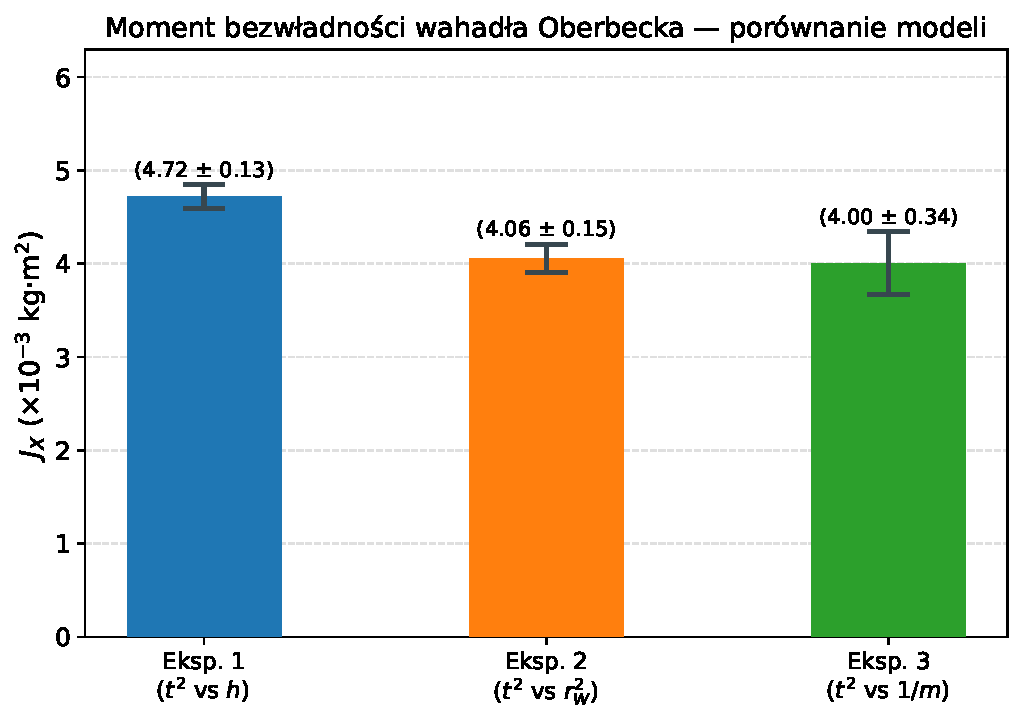
\includegraphics[width=0.82\textwidth]{wykres7_jx_porownanie.pdf}
    \caption{Porównanie wyznaczonych wartości $J_X$ z trzech eksperymentów. Słupki błędów odpowiadają niepewnościom rozszerzonymi ($k=1$).}\label{fig:jx_porownanie}
\end{figure}

\subsection{Zależność kwadratu czasu przelotu od odległości fotokomórek}
Wynik $J_X = (4{,}72 \pm 0{,}13)\times10^{-3}\ \si{\kg\m\squared}$ cechuje się najmniejszą niepewnością względną (${\approx}2{,}8\%$). Wysoki współczynnik determinacji $R^2 = 0{,}999$ potwierdza liniowość zależności $t^2(h)$.

Wyraz wolny $B_1 = (-3{,}98 \pm 0{,}84)\ \si{\s\squared}$ odbiega od zera o ${\approx}4{,}7\sigma$, co jest statystycznie istotne. Ujemna wartość $B_1$ wymaga osobnego komentarza. Tarcie i opory ruchu wydłużają czas przelotu i zwiększają $t^2$, co dałoby $B_1 > 0$ --- zatem tarcie nie może wyjaśniać obserwowanego ujemnego wyrazu wolnego. Natomiast $B_1 < 0$ jest spójne z systematycznym \emph{przeszacowaniem} odległości bramek $h$: jeśli rzeczywista odległość między wiązkami fotokomórek jest mniejsza o stałe $\delta$ od zmierzonej taśmą wartości $h$, to $t^2 = A_1(h - \delta) = A_1 h + B_1$, skąd $\delta = -B_1/A_1 \approx \qty{4{,}2}{\cm}$. Tak duży offset mógłby wynikać z mierzenia odległości między zewnętrznymi krawędziami obudów fotokomórek zamiast między ich wiązkami świetlnymi, lub z nieprawidłowego ustawienia punktu odniesienia taśmy mierniczej.

\subsection{Zależność kwadratu czasu przelotu od kwadratu odległości ciężarków od osi obrotu}
Wynik $J_X = (4{,}06 \pm 0{,}15)\times10^{-3}\ \si{\kg\m\squared}$ jest zgodny z eksperymentem~3 i mieści się w granicach $3\sigma$ od eksperymentu~1 ($|4{,}72 - 4{,}06|/\sqrt{0{,}13^2+0{,}15^2} \approx 3{,}3$). Moment bezwładności wyznaczono bezpośrednio z wyrazu wolnego $B_2$ i zmierzonej odległości bramek $h_2 = \qty{30.0 \pm 0.1}{\cm}$. Dominującym źródłem niepewności jest $u(B_2)$, odpowiadające za ${\approx}92\%$ wariancji $u^2(J_X)$; wkład $u(r)$ wynosi ${\approx}7\%$, pozostałe są pomijalne.

\subsection{Zależność kwadratu czasu przelotu od odwrotności masy ciężarków zawieszonych na nitce}
Wynik $J_X = (4{,}00 \pm 0{,}34)\times10^{-3}\ \si{\kg\m\squared}$ jest zgodny z eksperymentem~1 w granicach niepewności ($|4{,}72 - 4{,}00|/\sqrt{0{,}13^2+0{,}34^2} \approx 2{,}0$). Większa niepewność względna (${\approx}8{,}5\%$) wynika z silniejszego wpływu niepewności $u(h_3)$ przy wyznaczaniu $J_X$ ze współczynnika $A_3 \propto h_3$. Wyraz wolny $B_3 = (0{,}2 \pm 1{,}6)\ \si{\s\squared}$ jest zgodny z zerem, co potwierdza poprawność modelu~(\ref{eq:model3}).

% -------------------------------------------
\begin{thebibliography}{9}
\bibitem{skrypt}
\textit{Skrypt do ćwiczeń laboratoryjnych z fizyki, I Pracownia Fizyczna}, ćwiczenie M7.
\end{thebibliography}

\end{document}
% =============================================
